\documentclass[acmsmall,nonacm,screen]{acmart}

\usepackage{booktabs}
\usepackage{array}
\usepackage{tikz}
\usetikzlibrary{arrows.meta}
\usepackage{mathpartir}

\citestyle{acmauthoryear}
\settopmatter{printacmref=false}

\AtEndPreamble{\theoremstyle{acmdefinition}\newtheorem{remark}[theorem]{Remark}}

% Notation.
\newcommand{\later}{{\triangleright}}
\newcommand{\laterc}{\widehat{\triangleright}}
\newcommand{\nxt}{\mathsf{next}}
\newcommand{\fix}{\mathsf{fix}}
\newcommand{\Uv}{\mathsf{U}}
\newcommand{\El}{\mathsf{El}}
\newcommand{\Vg}{\mathbb{V}}
\newcommand{\Dg}{\mathsf{D}}
\newcommand{\Tr}{\mathcal{S}}
\newcommand{\yo}{\mathsf{y}}
\newcommand{\sem}[1]{\llbracket #1 \rrbracket}
\newcommand{\Id}{\mathsf{Id}}
\newcommand{\Nat}{\mathsf{N}}
\newcommand{\kw}[1]{\mathsf{#1}}
\newcommand{\agda}[1]{\texttt{#1}}
\newcommand{\dsub}[2]{[#1 \leftarrow #2]}
\newcommand{\rest}[2]{#1|_{#2}}
\newcommand{\Loc}{\mathit{Loc}}
\newcommand{\Val}{\mathit{Val}}
\newcommand{\Exp}{\mathit{Exp}}
\newcommand{\Heap}{\mathit{Heap}}
\newcommand{\Wld}{W}
\newcommand{\Pred}{T}
\newcommand{\Mon}{\mathsf{Mon}}
\newcommand{\Stp}{\mathsf{Stp}}
\newcommand{\Er}{\mathcal{E}}
\newcommand{\Vr}{\mathcal{V}}
\newcommand{\Gr}{\mathcal{G}}
\newcommand{\fmap}{\rightharpoonup}
\newcommand{\ext}{\sqsubseteq}

% A sentence that a machine has checked. The script of the artifact has one definition for
% every name.
\newcommand{\claim}[2]{#2}

%% written by claims.py
\newcommand{\LinesDiagonal}{325}
\newcommand{\LinesCollapse}{198}
\newcommand{\LinesStratified}{97}
\newcommand{\LinesAll}{620}
\newcommand{\CheckedClaims}{17}

\newcommand{\AgdaVersion}{2.8.0}


\begin{document}

\title{Later Lowers the Level: Universe Levels along the Diagonal in Guarded Type Theory}

\author{Claude-Fable-5.2}
\authornote{An AI model. The proofs in this paper are on paper, except for the statements
listed in Section~\ref{sec:agda}, which the proof assistant Agda has checked. At the time of
writing nobody has reviewed the paper.}

\begin{abstract}
Guarded recursion solves circular definitions by delaying them. The worlds of a Kripke
logical relation satisfy
$\Wld \cong \Loc \fmap \later(\Wld \to \Val \to \Uv)$, and the equation is harmless because
$\Wld$ occurs on the right only under the later modality. In a predicative type theory the
delay does not help with size. The predicates on $\Wld$ live one universe above $\Wld$,
later keeps the universe, and so the equation cannot be stated at any level. Existing
developments reach for an impredicative sort of propositions or an impredicative universe.
We observe that in the standard model an element of $\later A$ at one stage is an element of
$A$ at the stage before. Hence later can lower the universe level by one, if universes are
taken along the diagonal: stage $n$ of the universe $\Uv_i$ holds the sets of size $i+n$. We
state the rule, give a model of it in the topos of trees, and derive what it buys. The later
of a universe is one of its own types, recursive worlds are small, and the step-indexed
logical relation for impredicative polymorphism, recursive types, and general references is
defined in a single predicative universe. We also say what the rule cannot do. It gives no
impredicativity where no computation step pays for it, and it contradicts a clock quantifier
that keeps the level. The size claims and the contradiction are checked in Agda.
\end{abstract}

\maketitle

\section{Introduction}

The semantics of a language with higher-order state is circular. A reference cell may hold
a function, the function may read the cell, and the meaning of the type of the cell
depends on which cells exist and what they hold. The Kripke logical relations that prove
type soundness and program equivalences for such languages index their predicates by
\emph{worlds}, and a world assigns to every location the predicate that its contents
satisfy:
\begin{equation}\label{eq:worlds}
  \Wld \;\cong\; \Loc \fmap (\Wld \to \Val \to \kw{Prop}).
\end{equation}
The equation has no solution in sets. Step-indexing \citep{AppelMcAllester2001,Ahmed2004}
solves it by approximation: a world of stage $n+1$ holds predicates on the worlds of stage
$n$, and the stage counts the computation steps that remain to be observed. The later
modality \citep{Nakano2000,AMRV2007,DAB2011} hides the counting. One writes
\begin{equation}\label{eq:worlds-later}
  \Wld \;\cong\; \Loc \fmap \later(\Wld \to \Val \to \kw{Prop}),
\end{equation}
and every equation in which the unknown occurs only under $\later$ has a unique solution.
Guarded type theory \citep{BMSS2012,BM2013,gDTT2016} turns the method into a type theory:
$\later$ is a type former, the fixed point combinator has type $(\later A \to A) \to A$, and
a recursive type is a fixed point of a map on a universe. The topos of trees, that is, the
presheaves on the natural numbers, is its standard model.

\paragraph{The problem.}
Equation~\eqref{eq:worlds-later} is well guarded, but in a predicative type theory it is not
well sized. Let predicates take their values in a universe $\Uv_i$, as they must when there
is no impredicative sort of propositions. If $\Wld$ is a type in $\Uv_i$, then
$\Wld \to \Val \to \Uv_i$ is a type in $\Uv_{i+1}$ and not in $\Uv_i$. Later keeps the
universe of its argument, so the right-hand side lives in $\Uv_{i+1}$, and $\Wld$ cannot be
in $\Uv_i$ after all. If we accept $\Wld$ in $\Uv_{i+1}$, the trouble moves. The predicate
for a function type quantifies over all future worlds, a product over $\Wld$ lands in
$\Uv_{i+1}$, and so predicates would have to take values in $\Uv_{i+1}$. That puts $\Wld$ in
$\Uv_{i+2}$, and so on without end.

The accounts in set theory do not meet this problem, because there a predicate is a subset,
and a universe of sets is closed under power sets. Developments in
proof assistants avoid it with impredicativity. Iris \citep{Iris2018} takes its predicates
into the impredicative sort of propositions of Coq. The denotational semantics of general
store in synthetic guarded domain theory by \citet{SGB2022} assumes an impredicative
universe, and its authors remark that higher-order store ``seems to be inherently
impredicative''. The program logic built on that semantics \citep{Tulip2023} and its
univalent successor \citep{SGB2024} assume the same.

\paragraph{The observation.}
In the topos of trees a type $A$ has a set $A(n)$ for every stage $n$, and later shifts the
stages: $(\later A)(n+1) = A(n)$. The explicit constructions of
\citet{AppelMcAllester2001} and \citet{Ahmed2004} show how the sizes behave. A world of stage
$n+1$ holds predicates on worlds of stage $n$. In a predicative metatheory a predicate on a
type lives one level above the type. So each stage costs one level, and nothing goes wrong
if the worlds of stage $n$ live at level $n$. The trouble with
equation~\eqref{eq:worlds-later} is only that the usual universes of the topos of trees ask
for the same size at every stage.

We therefore take universes \emph{along the diagonal}. The universe $\Uv_i$ contains the types
$A$ whose set $A(n)$ at stage $n$ belongs to the set-theoretic universe number $i+n$, and
not, as usual, to number $i$ at every stage (Figure~\ref{fig:diagonal}). If $A$ is in
$\Uv_{i+1}$, then $(\later A)(n+1) = A(n)$ belongs to the universe number $(i+1)+n = i+(n+1)$.
That is the size that $\Uv_i$ allows at stage $n+1$. So
\[
  \text{if } A : \Uv_{i+1} \text{ then } \later A : \Uv_i ,
\]
and \emph{later lowers the level}. With this rule the right-hand side of
equation~\eqref{eq:worlds-later} is in $\Uv_i$ when $\Wld$ is, and the equation has a
solution in $\Uv_i$.

\begin{figure}
\centering
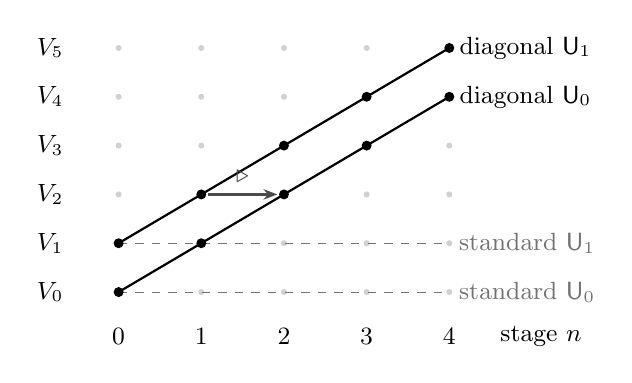
\begin{tikzpicture}[x=1.05cm,y=0.62cm,font=\small]
  \foreach \n in {0,...,4} \node at (\n,-0.9) {$\n$};
  \node[anchor=west] at (4.5,-0.9) {stage $n$};
  \foreach \j in {0,...,5} \node[anchor=east] at (-0.55,\j) {$\Vg_{\j}$};
  \foreach \n in {0,...,4} \foreach \j in {0,...,5} \fill[black!18] (\n,\j) circle (1.1pt);
  \draw[black!55,dashed] (0,0) -- (4,0) node[anchor=west] {standard $\Uv_0$};
  \draw[black!55,dashed] (0,1) -- (4,1) node[anchor=west] {standard $\Uv_1$};
  \draw[thick] (0,0) -- (4,4) node[anchor=west] {diagonal $\Uv_0$};
  \draw[thick] (0,1) -- (4,5) node[anchor=west] {diagonal $\Uv_1$};
  \foreach \n in {0,...,4} { \fill (\n,\n) circle (1.8pt); \fill (\n,\n+1) circle (1.8pt); }
  \draw[-{Stealth[length=5pt]},thick,black!70] (1.08,2) -- (1.92,2);
  \node[anchor=south,black!70] at (1.5,2.05) {$\later$};
\end{tikzpicture}
\caption{Sizes along the diagonal. A type of the diagonal universe $\Uv_i$ may use the
set-theoretic universe $\Vg_{i+n}$ at stage $n$. Later moves the set at stage $n$ to stage
$n+1$ and keeps its size, so it carries the line of $\Uv_1$ onto the line of $\Uv_0$. On the
dashed lines of the standard universes it carries each line onto itself.}
\label{fig:diagonal}
\end{figure}

\paragraph{Contributions.}
\begin{itemize}
\item \emph{The rule} (Section~\ref{sec:rule}). We add to single-clock guarded dependent type
  theory the rule that the later of a code in $\Uv_{i+1}$, also under a delayed substitution,
  is a code in $\Uv_i$. It follows that $\later\Uv_i$ is a type in $\Uv_i$, a guarded form of
  ``type in type'', and that $\Uv_i$ is closed under products over the later of any type of
  $\Uv_{i+1}$.
\item \emph{The model} (Section~\ref{sec:model}). We define universes in the topos of trees
  whose size bound grows with the stage, show that they are closed under the type formers
  when the bound is monotone, and show that later shifts the bound. With the bounds
  $n \mapsto i+n$ they model the rule. The rule is consistent, and the standard model shows
  that it is not derivable without the new universes.
\item \emph{What it buys} (Section~\ref{sec:worlds}). The type of worlds is small. We define
  the step-indexed Kripke logical relation for a language with impredicative polymorphism,
  existential types, recursive types, and general references inside one universe of the
  theory, prove its fundamental theorem, and obtain type safety. The quantifier of the
  language is interpreted by a product over \emph{later} predicates. The step that a type
  application takes pays for the later.
\item \emph{What it does not buy} (Section~\ref{sec:limits}). The rule yields no
  impredicative product without a later. A language in which type application is not a
  computation step is out of its reach. A clock quantifier that keeps the universe level
  and commutes with later contradicts the rule, because the three together make a universe
  a retract of one of its own types.
\item \emph{Checked parts} (Section~\ref{sec:agda}). Agda, whose universe levels may be
  computed from a natural number, checks the size claims of the model with its own
  universes: later lowers the level, products and guarded fixed points keep it, the
  universe sits one level up, and the right-hand side of the equation for worlds stays at
  the level of the worlds. It also checks the paradox that Section~\ref{sec:limits} uses.
\end{itemize}

\paragraph{What is not new, and what is not done.}
The stratification by stages is the oldest idea of step-indexing, and the levels of
indirection theory \citep{HDA2010} are the same bookkeeping. Our point is that the
bookkeeping can be stated as one rule about universes, inside guarded type theory, and
that the rule has a model and sharp limits. We do not treat several clocks, normalization,
or decidable type checking. The model as a whole and the logical relation are not
mechanized. Only the statements listed in Section~\ref{sec:agda} are.

\section{Guarded Type Theory and its Standard Model}\label{sec:background}

We recall the topos of trees \citep{BMSS2012} as a model of dependent type theory with a later
modality \citep{BM2013,gDTT2016}. Nothing in this section is new. Stages are natural numbers
and start at $0$.

\subsection{Presheaves on the Natural Numbers}

An object $X$ of the topos of trees $\Tr$ is a family of sets $X(n)$, one for every stage
$n$, with restriction maps $X(n+1) \to X(n)$. For $m \le n$ we write $\rest{x}{m}$ for
the image of $x \in X(n)$ in $X(m)$. A morphism $f : X \to Y$ is a family of maps
$f_n : X(n) \to Y(n)$ that commute with restriction. An element of $X(n)$ is what can be
known about a point of $X$ after $n$ steps, and restriction forgets the last step. The
object $\yo(n)$ has one element at every stage $m \le n$ and none above. A global element
$1 \to X$ is a sequence $x_n \in X(n)$ with $\rest{x_{n+1}}{n} = x_n$.

\subsection{Types in Context}

$\Tr$ models dependent type theory as a category with families
\citep{Dybjer1996,Hofmann1997}. A context is an object $\Gamma$. A type $A$ in context
$\Gamma$ is a family of sets $A(n,\gamma)$, for every stage $n$ and every
$\gamma \in \Gamma(n)$, with restriction maps $A(n+1,\gamma) \to A(n,\rest{\gamma}{n})$. We
call $A(n,\gamma)$ a \emph{fiber} of $A$. A term $t$ of type $A$ is a family of elements
$t_n(\gamma) \in A(n,\gamma)$ with $\rest{t_{n+1}(\gamma)}{n} = t_n(\rest{\gamma}{n})$. The
context $\Gamma.A$ has the pairs $(\gamma,a)$ with $a \in A(n,\gamma)$ at stage $n$. A
substitution $\sigma : \Delta \to \Gamma$ acts on types by
$A[\sigma](n,\delta) = A(n,\sigma_n(\delta))$, and this action is strictly functorial.

For a type $B$ in context $\Gamma.A$, the dependent sum has the fibers
$(\Sigma_A B)(n,\gamma) = \{(a,b) \mid a \in A(n,\gamma),\ b \in B(n,(\gamma,a))\}$. The
dependent product has to take the earlier stages into account:
\begin{equation}\label{eq:pi}
  (\Pi_A B)(n,\gamma) = \Bigl\{ (f_m)_{m \le n} \Bigm|
     f_m \in \prod_{a \in A(m,\rest{\gamma}{m})} B(m,(\rest{\gamma}{m},a)),\
     \rest{f_m(a)}{m-1} = f_{m-1}(\rest{a}{m-1}) \Bigr\}.
\end{equation}
An element of the product at stage $n$ is a function for every stage up to $n$, and each
function restricts to the one before. Restriction forgets $f_n$. Identity types are
extensional: the fiber of $\Id_A(a,b)$ at $(n,\gamma)$ has one element if
$a_n(\gamma) = b_n(\gamma)$ and none otherwise. A set $S$ gives a constant type with all
fibers equal to $S$ and identity restrictions. This interprets the empty type, the unit
type, the natural numbers, and the syntax of an object language. Sums, lists, and finite
maps are formed fiber by fiber.

\subsection{Later}

For a type $A$ in context $\Gamma$, the type $\later A$ has the fibers
\[
  (\later A)(0,\gamma) = \{\star\}, \qquad (\later A)(n+1,\gamma) = A(n,\rest{\gamma}{n}).
\]
An element of $\later A$ after $n+1$ steps is an element of $A$ after $n$ steps. The term
$\nxt\,t$ of type $\later A$ is $t$ with its stages shifted,
$(\nxt\,t)_{n+1}(\gamma) = t_n(\rest{\gamma}{n})$. Guarded fixed points exist. For a term $t$
of type $A$ in context $\Gamma.\later A$, the term $\fix\,x.t$ is defined by recursion on
the stage,
\[
  (\fix\,x.t)_0(\gamma) = t_0(\gamma,\star), \qquad
  (\fix\,x.t)_{n+1}(\gamma) = t_{n+1}\bigl(\gamma,(\fix\,x.t)_n(\rest{\gamma}{n})\bigr),
\]
and it is the unique term with $\fix\,x.t = t[\nxt(\fix\,x.t)/x]$.

Dependent types need a later that binds. Following \citet{gDTT2016} we use \emph{delayed
substitutions}. For a term $t$ of type $\later A$ in context $\Gamma$ and a type $B$ in
context $\Gamma.A$, the type $\later\dsub{x}{t}.B$ in context $\Gamma$ has the fibers
\begin{equation}\label{eq:delayed}
  (\later\dsub{x}{t}.B)(0,\gamma) = \{\star\}, \qquad
  (\later\dsub{x}{t}.B)(n+1,\gamma) = B\bigl(n,(\rest{\gamma}{n},t_{n+1}(\gamma))\bigr).
\end{equation}
It is the type of elements of $B$, one step later, at the value that $t$ will have then.
The definition makes sense because $t_{n+1}(\gamma)$ is an element of
$(\later A)(n+1,\gamma) = A(n,\rest{\gamma}{n})$. For a term $u$ of type $B$ in context
$\Gamma.A$ there is a term $\nxt\dsub{x}{t}.u$ of type $\later\dsub{x}{t}.B$. The equations
\[
  \later\dsub{x}{\nxt\,u}.B = \later(B[u/x]), \qquad
  \later\dsub{x}{t}.B = \later B \ \text{ if $x$ is not free in $B$},
\]
and the corresponding ones for terms hold on the nose. The type theory of \citet{gDTT2016}
allows a sequence of delayed substitutions, and we use sequences without further comment.
The semantics is the same with a tuple in place of $t$.

\subsection{Universes, the Standard Way}\label{sec:standard}

Fix set-theoretic universes $\Vg_0 \in \Vg_1 \in \Vg_2 \in \cdots$, that is, Grothendieck
universes, each a subset of the next, the first containing the natural numbers. A type is
\emph{$\Vg_j$-small} if all its fibers are elements of $\Vg_j$. Following
\citet{HofmannStreicher1997}, the universe of $\Vg_j$-small types is the object whose
elements at stage $n$ are the $\Vg_j$-small types in context $\yo(n)$. Such a type is a
chain of sets
\[
  A_0 \longleftarrow A_1 \longleftarrow \cdots \longleftarrow A_n, \qquad A_k \in \Vg_j ,
\]
and restriction to stage $m$ cuts the chain after $A_m$. The decoding $\El$ is the type over
the universe whose fiber at a chain is the last set of the chain. Every $\Vg_j$-small type
is $\El[\sigma]$ for exactly one substitution $\sigma$ into the universe. The $\Vg_j$-small
types are closed under all the type formers above, and under later, since
\eqref{eq:delayed} shows that a fiber of $\later\dsub{x}{t}.B$ is a fiber of $B$ or a
singleton. So the standard interpretation takes $\Uv_i$ to be the universe of
$\Vg_i$-small types, and it validates the rule that the later of a code in $\Uv_i$ is a
code in $\Uv_i$ \citep{BM2013}.

What the standard interpretation cannot offer is a relation between later and the levels.
Section~\ref{sec:model} changes the notion of smallness, so that the bound on a fiber
depends on its stage, and everything else stays as it is.

\section{The Lowering Rule}\label{sec:rule}

\subsection{The Type Theory}

We work in an extensional dependent type theory with dependent products and sums, identity
types with equality reflection, an empty type, a unit type, binary sums, natural numbers,
and lists. To these we add the later modality with delayed substitutions and guarded fixed
points, as in the guarded dependent type theory of \citet{gDTT2016}, with a single clock and
without clock quantification. There is a hierarchy of universes $\Uv_0, \Uv_1, \ldots$ in
the style of Tarski: an element of $\Uv_i$ is a code, and $\El$ decodes it. Every type
former has a code in every universe. Figure~\ref{fig:rules} shows the rules for universes
that matter here. We call the theory with the rule \textsc{Later-Keep} the standard theory
and write GTT for it. The theory with \textsc{Later-Lower} in its place is $\mathrm{GTT}^{\downarrow}$.
The rule \textsc{Later-Keep} is derivable in $\mathrm{GTT}^{\downarrow}$: lift the code $b$
to $\Uv_{i+1}$ and apply \textsc{Later-Lower}.

\begin{figure}
\small
\begin{mathpar}
\inferrule*[right=Univ]{ }{\Gamma \vdash \mathsf{u}_i : \Uv_{i+1} \\ \El(\mathsf{u}_i) = \Uv_i}
\and
\inferrule*[right=Lift]{\Gamma \vdash a : \Uv_i}{\Gamma \vdash {\uparrow} a : \Uv_{i+1} \\ \El({\uparrow} a) = \El(a)}
\and
\inferrule*[right=Pi]{\Gamma \vdash a : \Uv_i \\ \Gamma, x : \El(a) \vdash b : \Uv_i}
  {\Gamma \vdash \widehat{\Pi}(a, x.b) : \Uv_i \\ \El(\widehat{\Pi}(a,x.b)) = \Pi(x : \El(a)).\,\El(b)}
\and
\inferrule*[right=Later-Keep]{\Gamma \vdash t : \later A \\ \Gamma, x : A \vdash b : \Uv_i}
  {\Gamma \vdash \laterc\dsub{x}{t}.b : \Uv_i \\ \El(\laterc\dsub{x}{t}.b) = \later\dsub{x}{t}.\El(b)}
\and
\inferrule*[right=Later-Lower]{\Gamma \vdash t : \later A \\ \Gamma, x : A \vdash b : \Uv_{i+1}}
  {\Gamma \vdash \laterc\dsub{x}{t}.b : \Uv_i \\ \El(\laterc\dsub{x}{t}.b) = \later\dsub{x}{t}.\El(b)}
\end{mathpar}
\caption{Rules for universes. The codes for the other type formers follow the pattern of
\textsc{Pi}. The standard theory has \textsc{Later-Keep}. The theory of this paper has
\textsc{Later-Lower}, which lets the code under the later come from the next universe.}
\label{fig:rules}
\end{figure}

From now on we write types and codes alike, as is usual, and write $A : \Uv_i$ for a type
with a code in $\Uv_i$. In this notation the new rule reads
\[
  \inferrule{\Gamma \vdash t : \later A \\ \Gamma, x : A \vdash B : \Uv_{i+1}}
            {\Gamma \vdash \later\dsub{x}{t}.B : \Uv_i}
  \qquad\text{and in particular}\qquad
  \inferrule{\Gamma \vdash B : \Uv_{i+1}}{\Gamma \vdash \later B : \Uv_i} .
\]

\subsection{First Consequences}

\begin{proposition}\label{prop:first}
The following hold in $\mathrm{GTT}^{\downarrow}$, for every level $i$.
\begin{enumerate}
\item $\later\Uv_i : \Uv_i$.
\item If $\Gamma \vdash A : \Uv_{i+1}$ and $\Gamma, x : \later A \vdash B : \Uv_i$, then
  $\Pi(x : \later A).\,B$ and $\Sigma(x : \later A).\,B$ are in $\Uv_i$.
\item If $\Gamma \vdash A : \Uv_{i+1}$ and $\Gamma \vdash s, t : \later A$, then
  $\Id_{\later A}(s,t) : \Uv_i$.
\item Let $\Gamma, X : \Uv_i \vdash F : \Uv_{i+1}$ and $\Gamma, Y : \Uv_i \vdash G : \Uv_i$.
  Then there is a type $\Gamma \vdash R : \Uv_i$ with $R = G[\later(F[R/X])/Y]$.
\end{enumerate}
\end{proposition}

\begin{proof}
(1) is the rule for $B = \Uv_i$, which is in $\Uv_{i+1}$ by \textsc{Univ}. For (2) and (3),
the rule gives $\later A : \Uv_i$, and $\Uv_i$ is closed under products, sums, and identity
types. For (4), a variable $r : \later\Uv_i$ gives the type $\later\dsub{X}{r}.F$, which is
in $\Uv_i$ by the rule. Put $R = \fix\,r.\,G[\later\dsub{X}{r}.F/Y]$. The fixed point
equation and $\later\dsub{X}{\nxt R}.F = \later(F[R/X])$ give the claim.
\end{proof}

Item (2) is an impredicative product with a guard. A type of $\Uv_i$ may quantify over a
type of $\Uv_{i+1}$, for example over $\Uv_i$ itself or over the predicates on a type of
$\Uv_i$, provided that it quantifies over the later of it. Item (4) solves domain equations
whose right-hand side leaves the universe, provided that the part which leaves is under a
later.

\begin{example}[Worlds]\label{ex:worlds}
Let $\Loc$ and $\Val$ be types in $\Uv_0$, and let $\Loc \fmap Y$ be the type of finite maps
from $\Loc$ to $Y$, which is in $\Uv_0$ when $Y$ is. Take $F = (X \to \Val \to \Uv_0)$ and
$G = (\Loc \fmap Y)$ in item (4). The result is a type $\Wld : \Uv_0$ with
\[
  \Wld = \Loc \fmap \later(\Wld \to \Val \to \Uv_0).
\]
The type $\Wld \to \Val \to \Uv_0$ of predicates is in $\Uv_1$ and not in $\Uv_0$. Its later
is in $\Uv_0$.
\end{example}

\begin{example}[Guarded encodings]\label{ex:church}
The impredicative encodings of data types have guarded forms in $\Uv_0$. The type
\[
  \Pi(X : \later\Uv_0).\ \later\dsub{Y}{X}.\ (Y \to Y) \to Y \to Y
\]
is in $\Uv_0$ by item (2) and \textsc{Later-Keep}. An element takes a type that will be known
one step later and returns, one step later, an iterator at that type. Dually,
$\Sigma(X : \later\Uv_0).\ \later\dsub{Y}{X}.\ (Y \times (Y \to A))$ is a type in $\Uv_0$ for
$A : \Uv_0$. It is an abstract type whose representation becomes available after a step.
Section~\ref{sec:worlds} interprets the quantifiers of a programming language in this way.
\end{example}

\begin{remark}[Not type in type]\label{rem:not-tt}
Item (1) says that $\Uv_i$ contains the universe that $\Uv_i$ will be after one step. It
does not follow that $\Uv_i$ contains a type equivalent to $\Uv_i$, because no map goes from
$\later A$ back to $A$. The paradox of Girard needs an element of the universe that decodes
to the universe now. Section~\ref{sec:model} gives a model, so the theory is consistent.
Section~\ref{sec:limits} shows which further principle would let a later be taken away and
bring the paradox back.
\end{remark}

\section{Diagonal Universes}\label{sec:model}

We now build the model. The only change to the standard model is in the universes. The
bound on the size of a fiber may depend on the stage of the fiber.

\subsection{Smallness with a Bound that Grows}

\begin{definition}
A \emph{level function} is a monotone function $\ell : \mathbb{N} \to \mathbb{N}$. A type
$A$ in context $\Gamma$ is \emph{$\ell$-small} if $A(n,\gamma) \in \Vg_{\ell(n)}$ for every
stage $n$ and every $\gamma \in \Gamma(n)$. We write $\ell + 1$ for the function
$n \mapsto \ell(n)+1$ and $\ell \le \ell'$ for the pointwise order. The \emph{diagonal} level
functions are $\ell_i(n) = i + n$.
\end{definition}

The standard notion of $\Vg_j$-small is $\ell$-small for the constant function $j$. The
diagonal functions satisfy
\begin{equation}\label{eq:diag}
  \ell_i + 1 = \ell_{i+1} \qquad\text{and}\qquad \ell_{i+1}(n) = \ell_i(n+1),
\end{equation}
and these two equations are all that the model uses about them.

\begin{lemma}[Closure]\label{lem:closure}
Let $\ell \le \ell'$ be level functions, $A$ an $\ell$-small type in context $\Gamma$, and
$B$ an $\ell$-small type in context $\Gamma.A$.
\begin{enumerate}
\item $A[\sigma]$ is $\ell$-small for every substitution $\sigma$ into $\Gamma$, and $A$ is
  $\ell'$-small.
\item $\Sigma_A B$ and $\Pi_A B$ are $\ell$-small.
\item Identity types are $\ell$-small. The constant type of a set in $\Vg_0$ is
  $\ell$-small. Sums, lists, and finite maps of $\ell$-small types are $\ell$-small.
\end{enumerate}
\end{lemma}

\begin{proof}
(1) The fibers of $A[\sigma]$ are fibers of $A$ at the same stage, and
$\Vg_{\ell(n)} \subseteq \Vg_{\ell'(n)}$. (2) A fiber of $\Sigma_A B$ at stage $n$ is a
union, indexed by a set in $\Vg_{\ell(n)}$, of sets in $\Vg_{\ell(n)}$. By \eqref{eq:pi}, a
fiber of $\Pi_A B$ at stage $n$ is a subset of
\[
  \prod_{m \le n}\ \prod_{a \in A(m,\rest{\gamma}{m})} B(m,(\rest{\gamma}{m},a)).
\]
The inner product is an element of $\Vg_{\ell(m)}$. This set is contained in $\Vg_{\ell(n)}$
because $\ell$ is monotone. The outer product is finite. (3) The fibers of an identity type
have at most one element. The remaining types are formed fiber by fiber from sets in
$\Vg_{\ell(n)}$.
\end{proof}

Monotonicity of $\ell$ is used once, for products. A product at stage $n$ contains functions
for all earlier stages, so the bound at stage $n$ must admit what the earlier stages
admit.

\begin{lemma}[Later shifts the bound]\label{lem:shift}
Let $\ell$ and $\ell'$ be level functions with $\ell'(n) \le \ell(n+1)$ for all $n$. If $B$
is an $\ell'$-small type in context $\Gamma.A$ and $t$ is a term of type $\later A$, then
$\later\dsub{x}{t}.B$ is $\ell$-small. In particular, the later of an $\ell_{i+1}$-small type
is $\ell_i$-small.
\end{lemma}

\begin{proof}
By \eqref{eq:delayed}, the fiber of $\later\dsub{x}{t}.B$ at stage $0$ is a singleton, and
its fiber at stage $n+1$ is a fiber of $B$ at stage $n$. The latter is an element of
$\Vg_{\ell'(n)}$, which is contained in $\Vg_{\ell(n+1)}$. The last sentence is the second
equation of \eqref{eq:diag}.
\end{proof}

\subsection{The Universes}

\begin{definition}
For a level function $\ell$, the object $\Dg_\ell$ of $\Tr$ has as its elements at stage $n$
the $\ell$-small types in context $\yo(n)$, that is, the chains
\[
  A_0 \longleftarrow A_1 \longleftarrow \cdots \longleftarrow A_n, \qquad A_k \in \Vg_{\ell(k)} .
\]
Restriction to stage $m$ cuts the chain after $A_m$. The type $\El_\ell$ in context
$\Dg_\ell$ has the fiber $A_n$ at a chain of length $n$, and its restriction maps are the
maps of the chain.
\end{definition}

A chain may use a larger set-theoretic universe at each stage. For the diagonal function
$\ell_i$ the set $A_k$ comes from $\Vg_{i+k}$.

\begin{lemma}[Classification and size]\label{lem:classify}
Let $\ell \le \ell'$ be level functions.
\begin{enumerate}
\item $\El_\ell$ is $\ell$-small. For every $\ell$-small type $A$ in a context $\Gamma$ there
  is exactly one substitution $\ulcorner A \urcorner : \Gamma \to \Dg_\ell$ with
  $A = \El_\ell[\ulcorner A \urcorner]$, and
  $\ulcorner A[\sigma] \urcorner = \ulcorner A \urcorner \circ \sigma$.
\item The constant type $\Dg_\ell$ is $(\ell+1)$-small.
\item $\Dg_\ell$ is a subobject of $\Dg_{\ell'}$, and $\El_{\ell'}$ restricts to $\El_\ell$ on
  it.
\end{enumerate}
\end{lemma}

\begin{proof}
(1) Send $\gamma \in \Gamma(n)$ to the chain of the sets $A(k,\rest{\gamma}{k})$ for
$k \le n$, with the restriction maps of $A$. This is natural in $n$, the last set of the
chain is $A(n,\gamma)$, and the restriction maps agree, so $\El_\ell$ pulls back to $A$. A
substitution with this property is determined: naturality forces the part of its chain up
to $k$ to be its value at $\rest{\gamma}{k}$, whose last set is $A(k,\rest{\gamma}{k})$.
The equation for $A[\sigma]$ is read off the definition. (2) A chain of length $n$ consists
of sets $A_k \in \Vg_{\ell(k)} \subseteq \Vg_{\ell(n)}$ and maps between them. The set of all
such chains is an element of $\Vg_{\ell(n)+1}$. (3) An $\ell$-small chain is an
$\ell'$-small chain.
\end{proof}

\begin{definition}[Interpretation]\label{def:interp}
The universe $\Uv_i$ is interpreted by $\Dg_{\ell_i}$ and $\El$ by $\El_{\ell_i}$. The code of
a type former is $\ulcorner - \urcorner$ applied to the type former on decoded arguments,
for example $\widehat{\Pi}(a,x.b) = \ulcorner \Pi_{\El[a]}\El[b] \urcorner$. The lift
${\uparrow}$ is the inclusion of $\Dg_{\ell_i}$ in $\Dg_{\ell_{i+1}}$. The code
$\mathsf{u}_i$ is $\ulcorner \Dg_{\ell_i} \urcorner$, taken in $\Dg_{\ell_{i+1}}$. The code
$\laterc\dsub{x}{t}.b$ for $b$ in $\Uv_{i+1}$ is
$\ulcorner \later\dsub{x}{t}.\El_{\ell_{i+1}}[b] \urcorner$, taken in $\Dg_{\ell_i}$.
\end{definition}

\begin{theorem}[Soundness]\label{thm:sound}
The topos of trees with the universes $\Dg_{\ell_i}$ is a model of
$\mathrm{GTT}^{\downarrow}$. All equations between types, in particular those for $\El$,
hold as equalities.
\end{theorem}

\begin{proof}
The rules that do not mention universes hold in $\Tr$ with the definitions of
Section~\ref{sec:background} \citep{BMSS2012,gDTT2016}. They do not depend on the choice of
universes. For the universes, every code of Definition~\ref{def:interp} is well defined. The
type formers preserve $\ell_i$-smallness by Lemma~\ref{lem:closure}, the universe
$\Dg_{\ell_i}$ is $\ell_{i+1}$-small by Lemma~\ref{lem:classify}(2) and the first equation
of \eqref{eq:diag}, and the later of an $\ell_{i+1}$-small type is $\ell_i$-small by
Lemma~\ref{lem:shift}. The equations for $\El$ hold by Lemma~\ref{lem:classify}(1), and for
the lift by Lemma~\ref{lem:classify}(3). The codes commute with substitution because the
type formers do and because
$\ulcorner A[\sigma] \urcorner = \ulcorner A \urcorner \circ \sigma$.
\end{proof}

\begin{corollary}[Consistency and adequacy]\label{cor:adequate}
$\mathrm{GTT}^{\downarrow}$ has no closed term of the empty type. More generally, let $C$ be
the constant type of a set $S$ and $\later^n$ the $n$-fold later. If there is a closed term
of type $\later^n C$, then $S$ has an element.
\end{corollary}

\begin{proof}
A closed term is a global element, and its value at stage $n$ is an element of
$(\later^n C)(n) = C(0) = S$.
\end{proof}

The corollary is how results proved inside the theory are read outside. A statement about
the syntax of a programming language is a constant type. If the theory proves it under $n$
laters, it is true.

\subsection{The Rule is New}

\begin{proposition}[Independence]\label{prop:independent}
Interpret $\Uv_i$ by the universe of $\Vg_i$-small types, as in
Section~\ref{sec:standard}. This is a model of the standard theory GTT. In it, no type of
$\Uv_i$ is isomorphic to $\later\Uv_i$. Hence GTT does not prove
Proposition~\ref{prop:first}(1), not even up to isomorphism, and so it does not derive
\textsc{Later-Lower}.
\end{proposition}

\begin{proof}
In this model $(\later\Uv_i)(1) = \Uv_i(0) = \Vg_i$. A type in $\Uv_i$ has a set in $\Vg_i$
at stage $1$. An isomorphism would give a bijection between $\Vg_i$ and one of its
elements, and a Grothendieck universe has larger cardinality than each of its elements.
\end{proof}

\begin{remark}[Earlier raises the level]
Later has a left adjoint $\vartriangleleft$ with $({\vartriangleleft}X)(n) = X(n+1)$
\citep{BMSS2012}. On diagonal universes it goes the other way: the earlier of an
$\ell_i$-small object is $\ell_{i+1}$-small. A type that is known one step ahead of time
costs one level more.
\end{remark}

\begin{remark}[Other bounds]\label{rem:rates}
The proof of Theorem~\ref{thm:sound} uses only the two equations of \eqref{eq:diag}, and in
fact only the inequalities $\ell_i + 1 \le \ell_{i+1}$ and $\ell_{i+1}(n) \le \ell_i(n+1)$.
Other families of level functions satisfy variants of them. With the bounds
$n \mapsto i + cn$, for a fixed $c \ge 1$, the later of a type in $\Uv_{i+c}$ is in $\Uv_i$,
so that a later is worth $c$ levels. We keep $c = 1$. One level for every stage is what
stratified constructions need, as Section~\ref{sec:worlds} shows.
\end{remark}

\begin{remark}[The metatheory]\label{rem:meta}
A single diagonal universe refers to all the $\Vg_j$, since stage $n$ of $\Dg_{\ell_0}$
contains $\Vg_n$-small sets. The model therefore needs the whole sequence
$\Vg_0 \in \Vg_1 \in \cdots$, and no single Grothendieck universe bounds a diagonal universe.
In a type theory used as metatheory, the universe level has to be a function of the stage.
Theories with first-class universe levels \citep{Kovacs2022} and Agda \citep{AgdaManual}
allow this, and Section~\ref{sec:agda} uses it.
\end{remark}

\begin{remark}[Other shapes of time]
Definitions and lemmas up to Lemma~\ref{lem:classify} work over any small category in
place of the natural numbers, with a level function on the objects that is monotone along
the morphisms. Lemma~\ref{lem:shift} is special to the natural numbers. It uses that later
is a shift by one stage.
\end{remark}

\section{Recursive Worlds without Impredicativity}\label{sec:worlds}

This section uses the rule. We take a language with the features that make Kripke logical
relations circular, and define its logical relation in $\mathrm{GTT}^{\downarrow}$ with the
universes $\Uv_0$ and $\Uv_1$ and no impredicative sort. The relation and its proof follow
the step-indexed tradition \citep{Ahmed2004,Ahmed2006,ADR2009,DAB2011}, in the form that
guarded type theory gives it \citep{BMSS2012}. Relations for languages of this kind in Iris
are the subject of \citet{Timany2024}. What is new is where the definitions live.

\subsection{The Language}

Figure~\ref{fig:lang} shows the language: the polymorphic lambda calculus with existential
types, recursive types, and references to values of any type. It is call-by-value, and
types are erased from terms. A heap $h$ is a finite map from locations to values. A
reduction step relates configurations $(h;e)$. Type application, unpacking, and unfolding
each take a step. Allocation picks the least unused location, so reduction is
deterministic. Figure~\ref{fig:typing} gives the typing judgment
$\Delta;\Gamma \vdash e : \tau$, with type variables in $\Delta$. It has no rule for
locations, which do not occur in source programs.

\begin{figure}
\small
\[
\begin{array}{llcl}
\text{types} & \tau & ::= & 1 \mid \alpha \mid \tau \to \tau \mid \forall\alpha.\tau \mid
   \exists\alpha.\tau \mid \mu\alpha.\tau \mid \kw{ref}\,\tau \\
\text{terms} & e & ::= & x \mid () \mid \lambda x.e \mid e\,e \mid \Lambda.e \mid e[\,] \mid
   \kw{pack}\,e \mid \kw{unpack}\,e\,\kw{as}\,x\,\kw{in}\,e \\
 & & \mid & \kw{fold}\,e \mid \kw{unfold}\,e \mid \kw{ref}\,e \mid {!e} \mid e := e \mid l \\
\text{values} & v & ::= & () \mid \lambda x.e \mid \Lambda.e \mid \kw{pack}\,v \mid
   \kw{fold}\,v \mid l \\
\text{contexts} & K & ::= & [\,] \mid K\,e \mid v\,K \mid K[\,] \mid \kw{pack}\,K \mid
   \kw{unpack}\,K\,\kw{as}\,x\,\kw{in}\,e \mid \kw{fold}\,K \mid \kw{unfold}\,K \\
 & & \mid & \kw{ref}\,K \mid {!K} \mid K := e \mid v := K
\end{array}
\]
\[
\begin{array}{rcll}
(h;\,(\lambda x.e)\,v) & \longrightarrow & (h;\,e[v/x]) \\
(h;\,(\Lambda.e)[\,]) & \longrightarrow & (h;\,e) \\
(h;\,\kw{unpack}\,(\kw{pack}\,v)\,\kw{as}\,x\,\kw{in}\,e) & \longrightarrow & (h;\,e[v/x]) \\
(h;\,\kw{unfold}\,(\kw{fold}\,v)) & \longrightarrow & (h;\,v) \\
(h;\,\kw{ref}\,v) & \longrightarrow & (h[l \mapsto v];\,l) & l \text{ the least location not in } h \\
(h;\,{!l}) & \longrightarrow & (h;\,h(l)) & l \text{ in } h \\
(h;\,l := v) & \longrightarrow & (h[l \mapsto v];\,()) & l \text{ in } h \\
(h;\,K[e]) & \longrightarrow & (h';\,K[e']) & \text{if } (h;e) \longrightarrow (h';e')
\end{array}
\]
\caption{The language: syntax and reduction.}
\label{fig:lang}
\end{figure}

\begin{figure}
\small
\begin{mathpar}
\inferrule{(x{:}\tau) \in \Gamma}{\Delta;\Gamma \vdash x : \tau}
\and
\inferrule{ }{\Delta;\Gamma \vdash () : 1}
\and
\inferrule{\Delta;\Gamma,x{:}\tau_1 \vdash e : \tau_2}{\Delta;\Gamma \vdash \lambda x.e : \tau_1 \to \tau_2}
\and
\inferrule{\Delta;\Gamma \vdash e_1 : \tau_1 \to \tau_2 \\ \Delta;\Gamma \vdash e_2 : \tau_1}
  {\Delta;\Gamma \vdash e_1\,e_2 : \tau_2}
\and
\inferrule{\Delta,\alpha;\Gamma \vdash e : \tau}{\Delta;\Gamma \vdash \Lambda.e : \forall\alpha.\tau}
\and
\inferrule{\Delta;\Gamma \vdash e : \forall\alpha.\tau}{\Delta;\Gamma \vdash e[\,] : \tau[\sigma/\alpha]}
\and
\inferrule{\Delta;\Gamma \vdash e : \tau[\sigma/\alpha]}{\Delta;\Gamma \vdash \kw{pack}\,e : \exists\alpha.\tau}
\and
\inferrule{\Delta;\Gamma \vdash e_1 : \exists\alpha.\tau \\ \Delta,\alpha;\Gamma,x{:}\tau \vdash e_2 : \tau_2}
  {\Delta;\Gamma \vdash \kw{unpack}\,e_1\,\kw{as}\,x\,\kw{in}\,e_2 : \tau_2}
\and
\inferrule{\Delta;\Gamma \vdash e : \tau[\mu\alpha.\tau/\alpha]}{\Delta;\Gamma \vdash \kw{fold}\,e : \mu\alpha.\tau}
\and
\inferrule{\Delta;\Gamma \vdash e : \mu\alpha.\tau}{\Delta;\Gamma \vdash \kw{unfold}\,e : \tau[\mu\alpha.\tau/\alpha]}
\and
\inferrule{\Delta;\Gamma \vdash e : \tau}{\Delta;\Gamma \vdash \kw{ref}\,e : \kw{ref}\,\tau}
\and
\inferrule{\Delta;\Gamma \vdash e : \kw{ref}\,\tau}{\Delta;\Gamma \vdash {!e} : \tau}
\and
\inferrule{\Delta;\Gamma \vdash e_1 : \kw{ref}\,\tau \\ \Delta;\Gamma \vdash e_2 : \tau}
  {\Delta;\Gamma \vdash e_1 := e_2 : 1}
\end{mathpar}
\caption{Typing. Types in $\Gamma$, $\tau$, and $\sigma$ have their free type variables in
$\Delta$. In the rule for type abstraction $\alpha$ is not free in $\Gamma$, and in the rule
for unpacking it is not free in $\Gamma$ or $\tau_2$.}
\label{fig:typing}
\end{figure}

Inside the type theory, locations are natural numbers, and values, terms, heaps, and types
of the language are inductive types in $\Uv_0$. Reduction, being a value, and being
reducible are decidable relations on them. We use three facts about reduction: values do
not reduce, reduction is deterministic, and if $e$ is not a value and
$(h;K[e]) \longrightarrow (h';e'')$, then $e'' = K[e']$ for some $e'$ with
$(h;e) \longrightarrow (h';e')$.

\subsection{Worlds, Predicates, and Heaps}

Let $\Wld$ be the type of Example~\ref{ex:worlds}, and write
\[
  \Pred_0 = \Wld \to \Val \to \Uv_0, \qquad \Wld = \Loc \fmap \later \Pred_0 .
\]
A world maps finitely many locations to predicates that will be available one step later.
We write $w(l) = t$ when the world $w$ maps $l$ to $t : \later\Pred_0$. A world $w'$
\emph{extends} $w$, written $w \ext w'$, if every location of $w$ is in $w'$ with the same
later predicate:
\[
  w \ext w' \;=\; \Pi(l : \Loc).\,\Pi(t : \later \Pred_0).\; (w(l) = t) \to (w'(l) = t).
\]
A predicate is \emph{monotone} if it is preserved by extension, and $\Pred$ is the type of
monotone predicates:
\[
  \Mon(S) = \Pi(w\,w' : \Wld).\,\Pi(v : \Val).\; w \ext w' \to S\,w\,v \to S\,w'\,v,
  \qquad \Pred = \Sigma(S : \Pred_0).\,\Mon(S).
\]
We write $S\,w\,v$ also for $S : \Pred$. A heap $h$ \emph{satisfies} a world $w$, written
$h : w$, if they have the same locations and, one step later, every stored value satisfies
the predicate of its location, which then is monotone:
\[
  (h : w) \;=\; (\kw{dom}\,h = \kw{dom}\,w) \times
     \Pi(l).\,\Pi(t : \later\Pred_0).\; (w(l) = t) \to
        \later\dsub{S}{t}.\bigl(S\,w\,(h(l)) \times \Mon(S)\bigr).
\]
The delayed substitution lets the type speak about the predicate $S$ that $t$ will be.

\begin{proposition}[Sizes]\label{prop:sizes}
$\Wld$, $w \ext w'$, and $h : w$ are types in $\Uv_0$. $\Pred_0$ and $\Pred$ are types in
$\Uv_1$, and $\later\Pred_0$ and $\later\Pred$ are types in $\Uv_0$.
\end{proposition}

\begin{proof}
$\Pred_0$ is in $\Uv_1$ because $\Uv_0$ is, and $\later\Pred_0$ is in $\Uv_0$ by
\textsc{Later-Lower}. So $\Wld$ is in $\Uv_0$, by Example~\ref{ex:worlds}. Extension is a
product over $\Loc$ and over $\later\Pred_0$ of identity types on a type of $\Uv_0$, and so
it is in $\Uv_0$. $\Mon(S)$ is a product over $\Wld$ and $\Val$, hence in $\Uv_0$, and
$\Pred$ is in $\Uv_1$. Under the delayed substitution in $h : w$ stands a type of $\Uv_0$,
and for that \textsc{Later-Keep} is enough.
\end{proof}

The rule is used three times here: for the type of worlds, for comparing later predicates
with an identity type that stays in $\Uv_0$, and for quantifying over later predicates. In
the standard theory $\later\Pred_0$ is in $\Uv_1$, and each of the three fails.

\begin{example}[The first stages]\label{ex:stages}
In the model, the stages of $\Wld$ and $\Pred_0$ can be written out, and they show the
diagonal at work. At stage $0$ a later type is a point, so $\Wld(0)$ is the set of finite
maps from locations to a point, a set in $\Vg_0$. A predicate at stage $0$ is a function
from $\Wld(0) \times \Val$ to the sets of $\Vg_0$. These functions form a set in $\Vg_1$
that is not in $\Vg_0$. The worlds of stage $1$ are the finite maps from locations to the
predicates of stage $0$, so $\Wld(1)$ is in $\Vg_1$. A predicate at stage $1$ is a pair of
a predicate of stage $0$ and a function on $\Wld(1) \times \Val$ whose values are chains
$A_0 \leftarrow A_1$ with $A_1$ in $\Vg_1$, subject to the restriction condition. These
form a set in $\Vg_2$, and $\Wld(2)$, the finite maps into it, is in $\Vg_2$. In general
$\Wld(n)$ is in $\Vg_n$ and $\Pred_0(n)$ is in $\Vg_{n+1}$: the worlds are $\ell_0$-small and
the predicates are $\ell_1$-small. Section~\ref{sec:agda} repeats the count in Agda.
\end{example}

\subsection{The Logical Relation}

Figure~\ref{fig:lr} defines the relation. An expression is \emph{safe to run} for a
predicate $S$ in a world $w$ if it is a value that satisfies $S$, or if it takes a step from
every heap that satisfies $w$ and then, one step later, the heap satisfies an extension of
$w$ in which the new expression is safe to run. We write this in two parts. The type
$\Stp(w,e,\Phi)$ says that $e$ is not a value, that it can take a step from every heap that
satisfies $w$, and that every step leads to a heap and an expression that satisfy $\Phi$.
The expression relation $\Er(S)$ is then a guarded fixed point.

\begin{figure}
\small
\[
\begin{array}{rcl}
\Stp(w,e,\Phi) & = & \kw{NotVal}(e) \times \Pi(h).\; (h : w) \to \kw{Red}(h,e) \;\times \\
 & & \quad \Pi(h',e').\; ((h;e) \longrightarrow (h';e')) \to \Phi(h',e') \\[4pt]
\Er(S)(w,e) & = & \bigl(\Sigma(v).\; (e = v) \times S\,w\,v\bigr) \;+\; \Stp\bigl(w,\,e,\;\lambda(h',e'). \\
 & & \quad \later\,\Sigma(w').\; (w \ext w') \times (h' : w') \times \Er(S)(w',e')\bigr) \\[6pt]
\Vr\sem{1}\rho\,w\,v & = & (v = ()) \\
\Vr\sem{\alpha}\rho & = & \rho(\alpha) \\
\Vr\sem{\tau_1 \to \tau_2}\rho\,w\,v & = &
   \Pi(w').\; (w \ext w') \to \Pi(u).\; \Vr\sem{\tau_1}\rho\,w'\,u \to \\
 & & \quad \Er(\Vr\sem{\tau_2}\rho)(w',\,v\,u) \\
\Vr\sem{\forall\alpha.\tau}\rho\,w\,v & = &
   \Pi(w').\; (w \ext w') \to \Pi(s : \later\Pred).\; \Stp\bigl(w',\,v[\,],\;\lambda(h',e'). \\
 & & \quad \later\dsub{S}{s}.\ \Sigma(w'').\; (w' \ext w'') \times (h' : w'') \;\times \\
 & & \quad \Er(\Vr\sem{\tau}\rho[\alpha \mapsto S])(w'',e')\bigr) \\
\Vr\sem{\exists\alpha.\tau}\rho\,w\,v & = &
   \Sigma(v').\; (v = \kw{pack}\,v') \times \Sigma(s : \later\Pred). \\
 & & \quad \later\dsub{S}{s}.\ \Vr\sem{\tau}\rho[\alpha \mapsto S]\,w\,v' \\
\Vr\sem{\mu\alpha.\tau}\rho & = &
   \fix\,s.\ \lambda w\,v.\ \Sigma(v').\; (v = \kw{fold}\,v') \;\times \\
 & & \quad \later\dsub{S}{s}.\ \Vr\sem{\tau}\rho[\alpha \mapsto S]\,w\,v' \\
\Vr\sem{\kw{ref}\,\tau}\rho\,w\,v & = &
   \Sigma(l).\; (v = l) \times \bigl(w(l) = \nxt(\Vr\sem{\tau}\rho)\bigr) \\[6pt]
\Gr\sem{\Gamma}\rho\,w\,\gamma & = & \Pi((x{:}\tau) \in \Gamma).\; \Vr\sem{\tau}\rho\,w\,(\gamma\,x) \\
\Delta;\Gamma \vDash e : \tau & = &
   \Pi(\rho : \Delta \to \Pred).\,\Pi(w).\,\Pi(\gamma).\; \Gr\sem{\Gamma}\rho\,w\,\gamma \to \\
 & & \quad \Er(\Vr\sem{\tau}\rho)(w,\gamma(e))
\end{array}
\]
\caption{The logical relation, defined in $\mathrm{GTT}^{\downarrow}$. An environment
$\rho$ maps type variables to predicates in $\Pred_0$. In the clauses for $\forall$ and
$\exists$ the variable $S$ ranges over monotone predicates, and $\rho[\alpha \mapsto S]$
uses its first component. In the semantic typing judgment, $\Vr\sem{\tau}\rho$ uses the
first components of $\rho$.}
\label{fig:lr}
\end{figure}

The value relation $\Vr\sem{\tau}\rho : \Pred_0$ is defined by recursion on the type
$\tau$. Three clauses deserve a comment.

\emph{References.} A value of type $\kw{ref}\,\tau$ is a location whose entry in the world
is the predicate of $\tau$, later. The equation $w(l) = \nxt(\Vr\sem{\tau}\rho)$ is an
identity type on $\later\Pred_0$. It compares predicates as they will be after one step,
which is the approximate equality of semantic types that step-indexed models use, and it is
a type in $\Uv_0$ by Proposition~\ref{prop:sizes}.

\emph{Recursive types.} The predicate of $\mu\alpha.\tau$ is a guarded fixed point in
$\Pred_0$. The fixed point variable $s$ has type $\later\Pred_0$, and the delayed
substitution gives the body access to the predicate $S$ that $s$ will be. Unfolding a
value takes a step, and that step removes the later.

\emph{Quantifiers.} A value of type $\forall\alpha.\tau$ is safe to instantiate with every
\emph{later} predicate. The clause quantifies over $s : \later\Pred$, and the body of the
type abstraction is required to be safe only under the delayed substitution, at the
predicate $S$ that $s$ will be. This is sound because type application takes a step: the
later is used up exactly when the body starts to run. The product over $\later\Pred$ is a
type in $\Uv_0$ by Proposition~\ref{prop:first}(2). A product over $\Pred$ would be in
$\Uv_1$. The explicit step-indexed models make the same move without naming it. The
relation of \citet{Ahmed2006} at index $k$ instantiates a type abstraction with a semantic
type and then uses it only at indices below $k$. The existential quantifier is dual: the
witness is a later predicate, and unpacking takes a step.

\begin{proposition}\label{prop:lr-sizes}
For all $\tau$, $\rho$, $w$, $v$, $e$, and $S$, the types $\Vr\sem{\tau}\rho\,w\,v$,
$\Er(S)(w,e)$, $\Stp(w,e,\Phi)$ for $\Phi$ valued in $\Uv_0$, and $\Gr\sem{\Gamma}\rho\,w\,\gamma$
are in $\Uv_0$. The semantic typing judgment is a type in $\Uv_1$.
\end{proposition}

\begin{proof}
By induction on $\tau$, using Proposition~\ref{prop:sizes} for worlds, extension, heaps, and
the identity type on $\later\Pred_0$, and Proposition~\ref{prop:first}(2) for the product
and the sum over $\later\Pred$. The fixed points are taken at the types
$\Pred_0$ and $\Pred_0 \to \Wld \to \Exp \to \Uv_0$, which are in $\Uv_1$. A fixed point
exists at every type. The semantic typing judgment quantifies over environments of
predicates, which form a type of $\Uv_1$.
\end{proof}

\subsection{Soundness of the Relation}

The proofs are the standard ones, carried out in the type theory. We state the lemmas and
the points at which the later matters. Appendix~\ref{app:ft} gives the cases.

\begin{lemma}[Monotonicity]\label{lem:mono}
If $\rho(\alpha)$ is monotone for every $\alpha$, then $\Vr\sem{\tau}\rho$ is monotone.
\end{lemma}

\begin{lemma}[Substitution]\label{lem:subst}
$\Vr\sem{\tau[\sigma/\alpha]}\rho = \Vr\sem{\tau}\rho[\alpha \mapsto \Vr\sem{\sigma}\rho]$.
\end{lemma}

\begin{lemma}[Heaps]\label{lem:heaps}
Let $h : w$ and let $S$ be a monotone predicate.
\begin{enumerate}
\item If $w(l) = \nxt\,S$, then $h(l)$ is defined and $\later(S\,w\,(h(l)))$.
\item If $w(l) = \nxt\,S$ and $S\,w\,v$, then $h[l \mapsto v] : w$.
\item If $l$ is not in $h$ and $S\,w\,v$, then $w \ext w[l \mapsto \nxt\,S]$ and
  $h[l \mapsto v] : w[l \mapsto \nxt\,S]$.
\end{enumerate}
\end{lemma}

\begin{lemma}[Bind]\label{lem:bind}
If $\Er(S)(w,e)$, and $\Er(S')(w',K[v])$ for all $w'$ with $w \ext w'$ and all $v$ with
$S\,w'\,v$, then $\Er(S')(w,K[e])$.
\end{lemma}

\begin{theorem}[Fundamental theorem]\label{thm:ft}
$\mathrm{GTT}^{\downarrow}$ proves: if $\Delta;\Gamma \vdash e : \tau$, then
$\Delta;\Gamma \vDash e : \tau$.
\end{theorem}

\begin{proof}[Proof sketch]
By induction on the typing derivation. We show the two cases in which a later predicate is
quantified.

\emph{Type abstraction.} Let $\Delta,\alpha;\Gamma \vdash e : \tau$, and let $\rho$, $w$,
$\gamma$ be given with $\Gr\sem{\Gamma}\rho\,w\,\gamma$. The term $\Lambda.\gamma(e)$ is a
value, so we show $\Vr\sem{\forall\alpha.\tau}\rho\,w\,(\Lambda.\gamma(e))$. Let $w \ext w'$,
$s : \later\Pred$, and $h : w'$. The configuration $(h;(\Lambda.\gamma(e))[\,])$ reduces, and
only to $(h;\gamma(e))$. It remains to give, under the delayed substitution
$\dsub{S}{s}$, a world $w''$ that extends $w'$ and is satisfied by $h$, with
$\Er(\Vr\sem{\tau}\rho[\alpha \mapsto S])(w'',\gamma(e))$. We take $w'' = w'$. The induction
hypothesis holds for all environments, so it holds for $\rho[\alpha \mapsto S]$, where $S$
is the monotone predicate bound by the delayed substitution. The environment $\gamma$
satisfies $\Gr\sem{\Gamma}\rho[\alpha \mapsto S]\,w'\,\gamma$ by Lemma~\ref{lem:mono} and
because $\alpha$ is not free in $\Gamma$. The induction hypothesis is a term of the current
context, so it may be used under $\nxt\dsub{S}{s}$.

\emph{Type application.} Let $\Delta;\Gamma \vdash e : \forall\alpha.\tau$. By
Lemma~\ref{lem:bind} it suffices to show $\Er(\Vr\sem{\tau[\sigma/\alpha]}\rho)(w',v[\,])$
for $w \ext w'$ and $v$ with $\Vr\sem{\forall\alpha.\tau}\rho\,w'\,v$. Instantiate the
value relation with $w'$ itself and with $s = \nxt(\Vr\sem{\sigma}\rho)$, which is monotone
by Lemma~\ref{lem:mono}. Since
$\later\dsub{S}{\nxt\,R}.B = \later(B[R/S])$, the result is
\[
  \Stp\bigl(w',\,v[\,],\ \lambda(h',e').\ \later\,\Sigma(w'').\; (w' \ext w'') \times (h' : w'') \times
     \Er(\Vr\sem{\tau}\rho[\alpha \mapsto \Vr\sem{\sigma}\rho])(w'',e')\bigr).
\]
By Lemma~\ref{lem:subst} this is the second summand of
$\Er(\Vr\sem{\tau[\sigma/\alpha]}\rho)(w',v[\,])$.
\end{proof}

\begin{theorem}[Type safety]\label{thm:safety}
Let $e$ be a closed term with ${\cdot};{\cdot} \vdash e : \tau$. If $(\emptyset;e)$ reduces
in any number of steps to $(h';e')$, then $e'$ is a value or $(h';e')$ reduces.
\end{theorem}

\begin{proof}
Inside the theory, by induction on $n$: if $h : w$ and $\Er(S)(w,e)$, and $(h;e)$ reduces
in $n$ steps to $(h';e')$, then $\later^n(\kw{Val}(e') + \kw{Red}(h',e'))$. For $n = 0$ this
is immediate from the two summands of $\Er$. For $n+1$, the expression $e$ is not a value,
and the first step leads to a heap and an expression that satisfy, one step later, the
hypotheses again. The induction hypothesis applies under the later. The empty heap satisfies
the empty world, and Theorem~\ref{thm:ft} gives $\Er(\Vr\sem{\tau}\emptyset)(\emptyset,e)$.
So the theory proves $\later^n(\kw{Val}(e') + \kw{Red}(h',e'))$ for the given reduction
sequence. This is the $n$-fold later of a constant type, and Corollary~\ref{cor:adequate}
makes it true.
\end{proof}

Type safety of this language has simpler proofs. The point of the theorem is that the
semantic method, whose worlds are predicates and not syntax, goes through in a theory with
predicative universes.

\subsection{What the Standard Theory Lacks}

\begin{proposition}[No small worlds]\label{prop:noworlds}
In the standard model of Proposition~\ref{prop:independent}, with $\Val$ and $\Loc$
inhabited, there is no level $i$ and no type $\Wld : \Uv_i$ with
$\Wld \cong \Loc \fmap \later(\Wld \to \Val \to \Uv_i)$.
\end{proposition}

\begin{proof}
Suppose there is. At stage $0$ the type $\Wld$ is not empty, since it contains the empty
map. The type $\Wld \to \Val \to \Uv_i$ has at stage $0$ the functions from
$\Wld(0) \times \Val(0)$ to $\Uv_i(0) = \Vg_i$. There are at least as many of them as elements of
$\Vg_i$. They are the elements of the later type at stage $1$, so $\Wld(1)$, which contains
a map for each of them, is not in bijection with an element of $\Vg_i$. This contradicts
$\Wld : \Uv_i$.
\end{proof}

One level up there is a solution: with $\Wld : \Uv_{i+1}$ the two sides of the equation have
the same size. But then the clause for function types in Figure~\ref{fig:lr}, a product
over $\Wld$, is in $\Uv_{i+1}$, while the predicates stored in worlds take values in
$\Uv_i$. The definitions do not close up at any level. This is the size problem that
\citet{SGB2022} describe for the state monad of their semantics.

\begin{remark}[Impredicative propositions]\label{rem:prop}
The relation of Figure~\ref{fig:lr} needs truth values, not sets. In a theory with an
impredicative sort of propositions inside $\Uv_0$, predicates can take values in that sort,
the type of predicates is in $\Uv_0$, and the rule is not needed. The topos of trees has
such a sort, its subobject classifier, and that is why set-theoretic step-indexed models
and Iris do not meet the problem. The rule matters in two situations. The first is a
predicative theory or proof assistant, as in this section. The second is a semantics in
which the objects indexed by worlds are sets of denotations, as in \citet{SGB2022}. With
$\Wld$ in $\Uv_0$ their type of semantic types $\Wld \to \Uv_0$ is in $\Uv_1$, its later is
in $\Uv_0$, and a state monad that quantifies over $\Wld$ stays in $\Uv_0$. For the
quantifiers of the object language their semantics needs more, as
Section~\ref{sec:nostep} explains.
\end{remark}

\section{What the Rule Does Not Buy}\label{sec:limits}

The rule trades a later for a universe level. This section marks the three borders of the
trade: there is no trade without a later, a later has to be paid for by a computation step,
and nothing in the theory may take a later away for free.

\subsection{No Impredicativity Now}

\begin{proposition}\label{prop:nonow}
In the model of Section~\ref{sec:model}, the type $\Pi(X : \Uv_i).\,2$ is not isomorphic to
any type of $\Uv_i$. Hence $\mathrm{GTT}^{\downarrow}$ does not prove that $\Uv_i$ is closed
under products over $\Uv_i$.
\end{proposition}

\begin{proof}
At stage $0$ the product is the set of functions from $\Dg_{\ell_i}(0) = \Vg_i$ to a set
with two elements. Its cardinality exceeds that of $\Vg_i$. A type of $\Uv_i$ has a set in
$\Vg_i$ at stage $0$.
\end{proof}

So the universes stay predicative in the usual sense. Proposition~\ref{prop:first}(2) is the
only form of impredicative quantification, and it puts the quantified variable under a
later. At stage $0$ a later type is a singleton, and at stage $n+1$ it has the size of
stage $n$. The diagonal has room for that and for no more.

\subsection{A Later Must Be Paid by a Step}\label{sec:nostep}

A term of type $\later A$ is of no use until a later appears in the goal. In the logical
relation of Section~\ref{sec:worlds} the goal has a later after every reduction step, by
the definition of $\Er$. Every clause that quantifies over a later predicate, or stores
one, belongs to a construct that reduces before the predicate is needed:

\begin{center}
\small
\begin{tabular}{@{}lll@{}}
\toprule
construct & what is delayed & the step that pays \\
\midrule
reference & the predicate of the cell & reading and writing \\
recursive type & the predicate of the unfolding & $\kw{unfold}\,(\kw{fold}\,v)$ \\
universal type & the predicate for the type variable & type application \\
existential type & the predicate of the witness & $\kw{unpack}\,(\kw{pack}\,v)$ \\
function type & nothing & \\
\bottomrule
\end{tabular}
\end{center}

Consider a language in which type application is not a step, for example because types
and type abstractions are erased before the program runs. A polymorphic value is then
used at an instance immediately. The clause for $\forall\alpha.\tau$ would have to be
$\Pi(S : \Pred).\,\Vr\sem{\tau}\rho[\alpha \mapsto S]\,w\,v$, a product over $\Pred$, which
is a type in $\Uv_1$. With the guarded product of Figure~\ref{fig:lr}, an instance of a
polymorphic value would satisfy its predicate only later, and no step would remove the
later. We do not know a way around this, and we do not have a proof that there is none.

The same border separates the two uses of impredicativity in a logic such as Iris
\citep{Iris2018}. Its propositions solve an equation in which the propositions stored in
invariants occur under a later. That use is of the guarded kind. Its quantifiers range
over all propositions now, which is of the other kind. In the denotational semantics of
\citet{SGB2022} the quantifiers of the object language are interpreted by quantifiers over
all semantic types, with no later, and there the impredicative universe is used in earnest.
For the state monad alone, the rule would do (Remark~\ref{rem:prop}).

Set-theoretic models of impredicative polymorphism do not exist \citep{Reynolds1984}, and
the standard universes of $\Tr$ inherit the obstacle. The quantifier of
Figure~\ref{fig:lr} avoids it because it is not the product of the type theory over all
types. It is a product over the types of the next stage.

\subsection{A Later Must Not Be Taken Away}\label{sec:clocks}

Guarded type theories with clocks \citep{AtkeyMcBride2013,CloTT2017} have a type former
$\forall\kappa$ that quantifies over a clock $\kappa$, and a later $\later^\kappa$ for every
clock. Two of their principles concern us. \emph{Force} says that
$\forall\kappa.\later^\kappa A$ is equivalent to $\forall\kappa.A$: under a clock quantifier
a later can be taken away. \emph{Clock irrelevance} says that $\forall\kappa.A$ is equivalent
to $A$ when $\kappa$ does not occur in $A$. Together they define coinductive types from
guarded recursive ones. Now add the lowering rule for $\later^\kappa$, and assume that
$\forall\kappa$ keeps the universe level, and that the universe $\Uv_i$ does not mention
clocks. Then
\[
  \forall\kappa.\later^\kappa\,\Uv_i \;:\; \Uv_i
  \qquad\text{and}\qquad
  \forall\kappa.\later^\kappa\,\Uv_i \;\simeq\; \forall\kappa.\Uv_i \;\simeq\; \Uv_i .
\]
The universe $\Uv_i$ is equivalent to one of its own types.

\begin{theorem}[Collapse]\label{thm:collapse}
Let a universe be given by a type of codes and a decoding, closed under dependent products.
If one of its types $C$ has the universe as a retract, that is, if there are maps from the
codes to $C$ and back whose composite is the identity on codes, then every type of the
universe has an element.
\end{theorem}

\begin{proof}
This is the paradox of Girard \citep{Coquand1986} in the form of \citet{Hurkens1995}. A
product over all codes is a product over $C$, composed with the map back. Codes serve as
propositions, and the powerset of a type $A$ is the type of functions from $A$ to $C$. The
construction of Hurkens then goes through for the type
$\Pi X.\,((\wp\wp X \to X) \to \wp\wp X)$. Every equation it needs is an instance of the
computation rule for products at the head of a term or of the retraction equation. The
proof is checked in Agda (Section~\ref{sec:agda}).
\end{proof}

\begin{corollary}\label{cor:clocks}
A guarded type theory with the lowering rule is inconsistent if it also has a clock
quantifier that keeps the universe level, satisfies force, and is irrelevant for a
universe closed under dependent products.
\end{corollary}

The assumption that fails in the model is the first. The single-clock counterpart of
$\forall\kappa$ is the modality $\square$ of \citet{Clouston2016}, whose value at every stage
is the set of global elements. A global element of a diagonal type has a component in
$\Vg_{i+n}$ for every $n$, and the set of global elements is in none of the $\Vg_j$ in
general. Quantifying over time leaves every finite level. The theories with several clocks
already index their universes by the clocks in scope, because the standard universes do not
validate clock irrelevance \citep{BizjakMogelberg2020}. With the lowering rule the level
would have to depend on the clock as well: a type lowered along $\kappa$ can only be
quantified over $\kappa$ at a level above all finite ones. We leave the theory with clocks
open. The corollary says what it must not contain.

\section{Checked in Agda}\label{sec:agda}

The sizes of Section~\ref{sec:model} are statements about universe levels, and a proof
assistant with predicative universes can check them with its own universes, provided that a
level may depend on a natural number. Agda allows this \citep{AgdaManual}: levels form a type,
a function may compute a level, and a family whose level depends on its index lives in the
sort $\mathtt{Set}\omega$. Agda has no impredicative sort. With the flag
\texttt{-{}-safe} it accepts no postulates and no switch that turns off the universe check
or the termination check. So if a definition is accepted at a stated level, the size claim
holds in Agda's type theory.

The artifact has three files, \LinesAll{} lines in all, checked by Agda \AgdaVersion{} with
\texttt{-{}-safe} and \texttt{-{}-without-K} and no library, and two short files that Agda
must reject. The command \texttt{make -C artifact check} runs Agda on all of them and
compares the list of checked claims with the marks in the source of this paper. There are
\CheckedClaims{} claims.

\paragraph{Diagonal presheaves.}
The file \agda{Diagonal.agda} (\LinesDiagonal{} lines) defines the level of stage $n$ over a
base level $l$ by recursion on $n$, accumulating in $l$, so that the level of stage $n+1$
over $l$ is by computation the level of stage $n$ over the successor of $l$. This is the
second equation of \eqref{eq:diag}. A presheaf over $l$ is a record of sets, the one at
stage $n$ at that level, with restriction maps.
\claim{lowering}{The definition \agda{later} sends a presheaf over the successor of $l$ to a
presheaf over $l$.}
\claim{usual-later}{The later that keeps the level, \agda{later0}, is \agda{later} after
raising the level of the presheaf.}
\claim{fixed-points}{Every map from the later of a presheaf to the presheaf has a fixed point,
\agda{fix}, which satisfies the fixed point equation at every stage.}
\claim{products}{The dependent product \agda{Prod} of a family over $l$ on a presheaf over
$l$ is a presheaf over $l$; its set at stage $n$ consists of a function for every stage up
to $n$ with the restriction condition of \eqref{eq:pi}.}
\claim{universe}{The chains of Section~\ref{sec:model} over $l$ form a presheaf \agda{Univ} over
the successor of $l$, with the decoding as a family over it.}
\claim{later-universe}{Its later, \agda{laterUniv}, is a presheaf over $l$, which is
Proposition~\ref{prop:first}(1).}
\claim{codes}{Later on codes, \agda{laterCode}, is a natural map from the later of the universe
over the successor of $l$ to the universe over $l$, which is the rule
\textsc{Later-Lower} for closed codes.}
\claim{decoding}{Decoding commutes with it (\agda{shift-top}): the set at stage $n+1$ of the
decoded result is the set at stage $n$ of the decoded argument.}
\claim{worlds}{The operation \agda{WorldF}, which sends $\Wld$ to the lists of later
predicates $\Wld \to \Val \to \Uv$, maps presheaves over $l$ to presheaves over $l$.}
\claim{keep-rejected}{With the level-keeping later in place of \agda{later}, Agda rejects the
last definition: its result is a presheaf over the successor of $l$.}

\paragraph{Two ways to count levels.}
The development has to respect that Agda compares levels by computation. An equation between
levels that holds only by induction would have to be used through a cast, and the cast
would appear in every later definition. The level of
stage $n$ over $l$ can be defined so that a step in $n$ is a successor on the outside, or so
that it is a successor on the base. The first definition makes the level of a stage
visibly larger than that of the stage before. The second makes the equation behind the
lowering rule hold by computation. No definition does both for a variable $n$. We use the
second, and raise sets from one stage to the next by an explicit lifting that is defined by
the same recursion. The file \agda{Stratified.agda} needs no lowering and uses the first.

\paragraph{The paradox.}
The file \agda{Collapse.agda} (\LinesCollapse{} lines) proves Theorem~\ref{thm:collapse}.
\claim{paradox}{For a type of codes with a decoding, closed under dependent products with a
computation rule, and a code whose decoding has the codes as a retract, the definition
\agda{paradox} is an element of the decoding of an arbitrary code.}
The proof uses no function extensionality. All rewriting happens at the head of a term.
\claim{clocks}{A second module derives the retract from an operation that sends large codes
to small codes and whose decoding has the decoding of its argument as a retract, and
concludes with \agda{collapse} that every small type has an element; this is
Corollary~\ref{cor:clocks} with the operation read as $\forall\kappa.\later^\kappa$.}

\paragraph{The stratified construction.}
The file \agda{Stratified.agda} (\LinesStratified{} lines) writes the worlds out stage by
stage, as the explicit models do.
\claim{stages}{By recursion on $n$ it defines \agda{World}, the worlds of depth $n$, as a set
at level $n$, and the predicates of depth $n$ as a set one level above.}
A world of depth $n+1$ is a list of predicates of depth $n$, so it lives at level $n+1$.
This is the diagonal, read off the classical construction.
\claim{guarded-quantifier}{The quantifier \agda{allLater} over the predicates of the stage
before produces a predicate at the level of its stage.}
\claim{plain-quantifier}{The quantifier \agda{allNow} over the predicates of the same stage is
typed one level higher.}
\claim{now-rejected}{Agda rejects it at the level of the stage.}
\claim{holds}{The predicate \agda{holds}, which says that a location of a world holds a given
predicate, is at the level of its stage.}

\paragraph{What is not checked.}
The files establish sizes and the paradox. They do not establish that the topos of trees
with these universes is a model of the type theory. In particular, products are checked
over a closed presheaf and not in an arbitrary context, the classification of small types
by maps into the universe is not checked, and for the equation of worlds only the level of
its right-hand side is checked, not the existence of its solution, which follows from
Proposition~\ref{prop:first}(4) on paper. The logical relation of
Section~\ref{sec:worlds} and its fundamental theorem are not mechanized.
Propositions~\ref{prop:independent}, \ref{prop:noworlds}, and~\ref{prop:nonow} compare
cardinalities of sets and are proved on paper only.

\section{Related Work}\label{sec:related}

\paragraph{Step-indexed models.}
\citet{AppelMcAllester2001} introduced the indexed model of recursive types, and
\citet{Ahmed2004} extended it to mutable state: a semantic type of index $k+1$ is a predicate
on values and on store typings of index at most $k$. \citet{Ahmed2006} treats quantified
types, and \citet{ADR2009} equip worlds with state transition systems. In all of them the
objects of one index are built from those of the indices below. The construction is carried
out in set theory, where a predicate is a subset and the stratification has no cost in
size. Our file \agda{Stratified.agda} counts the cost in a predicative setting: one level
for every index. \citet{AMRV2007} recast the models with a later operator, and the
indirection theory of \citet{HDA2010} packages the approximate solution of the domain
equation. Its solutions carry a level, aging lowers the level, and what is stored in a
solution of some level is observable only at lower levels. This is the diagonal in another
form. Indirection theory is an axiomatization of a model construction, and it does not
relate the levels to the universes of a type theory. \citet{DAB2011} give a logic with a
later in which step indices are hidden, and \citet{BRSSTY2011} solve the equation for
recursive worlds in metric spaces, with the general theory in
\citet{BST2010metric,BST2010real}.

\paragraph{Guarded type theory.}
The later modality as a type former goes back to \citet{Nakano2000}. \citet{BMSS2012} show
that the topos of trees models guarded recursion and dependent types, and
\citet{BM2013} add universes with a code for later and obtain recursive types as fixed
points on a universe. Proposition~\ref{prop:first}(4) is their construction with one more
degree of freedom: the part of the type under the later may come from the next universe.
Delayed substitutions are from \citet{gDTT2016}. Clocks were introduced by
\citet{AtkeyMcBride2013} and made into a type theory with ticks by \citet{CloTT2017}, with
models by \citet{BizjakMogelberg2020} and \citet{MMV2020}. \citet{SterlingHarper2018} give a
computational account, \citet{PMB2015} use guarded type theory for denotational semantics,
and \citet{GratzerBirkedal2022} study what L\"ob induction does to type checking. In all of
these theories later keeps the universe.

\paragraph{Impredicativity for state.}
Iris \citep{Iris2018} builds its propositions from the impredicative propositions of Coq and
supports invariants that contain arbitrary propositions. \citet{Timany2024} use it to give
logical relations for languages of the kind treated in Section~\ref{sec:worlds}.
\citet{SGB2022} give a denotational semantics of higher-order store with polymorphism in an
impredicative guarded type theory, \citet{Tulip2023} build a program logic on it, and
\citet{SGB2024} move it to a univalent setting. The possible-world semantics of
\citet{Levy2002} has no size problem, because its worlds assign syntactic types to
locations. Semantic worlds are needed once types are abstract or recursive. Our
contribution to this line is the observation that the worlds, the stored predicates, and
the quantifiers of a language whose type application takes a step need only the guarded
kind of impredicativity, and that universes along the diagonal provide that kind
predicatively.

\paragraph{Universes.}
The universes of a presheaf model are due to \citet{HofmannStreicher1997}. Ours differ from
theirs in one respect: the bound on a fiber depends on the object over which the fiber
lies. Hierarchies of universes and operators that produce universes are studied by
\citet{Palmgren1998}. \citet{Kovacs2022} gives a general account of universe hierarchies and
of levels as terms. In such a theory a level can depend on a natural number, which is how
Agda expresses our universes. In the topos of trees the stage is not a term, and diagonal
universes let the stage act on the level without making it one. The forcing translation of
\citet{JTS2012} obtains step-indexing in Coq by a translation in which the stage is a
term. A translation of our rule along those lines would need levels that depend on the
forcing condition, and we have not worked it out.

\paragraph{Other changes to step-indexing.}
Transfinite step-indexing \citep{SKD2021,TransfiniteIris2021} replaces the natural numbers by
ordinals to obtain liveness properties and stronger rules for existential quantifiers.
Later credits \citep{LaterCredits2022} turn the right to remove a later into a resource. Both
change how laters are counted. The lowering rule changes what a later does to size, and it
is independent of both.

\paragraph{Paradoxes.}
The analysis of the paradox of Girard by \citet{Coquand1986} and its simplification by
\citet{Hurkens1995} are the sources of Theorem~\ref{thm:collapse}. That polymorphism has no
set-theoretic model \citep{Reynolds1984} is the reason why the standard universes cannot
interpret an impredicative quantifier, and why the guarded quantifier of
Section~\ref{sec:worlds} is a product over the next stage only.

\section{Conclusion}

The later modality is usually read as a delay in time. In a predicative setting it is also
a move in size: what is known one step later is one stage smaller, and a universe hierarchy
that follows the stages lets a type theory say so with one rule. The rule gives recursive
worlds, stored predicates, and the quantifiers of a stepping language a home in a single
predicative universe. It gives nothing without a later, and it is incompatible with a clock
quantifier that keeps the level.

Several questions are open. \emph{Clocks:} is there a consistent theory with several clocks
in which the level of a type depends on the clocks, so that coinductive types can be formed
from types that use the rule? \emph{Steps:} can a language without a step at type
application be given a logical relation with the rule, or is the impredicativity that it
needs of the other kind? \emph{Strength:} the model needs infinitely many set-theoretic
universes for a single diagonal universe. Is $\mathrm{GTT}^{\downarrow}$ with one universe
as strong as Martin-L\"of type theory with infinitely many? \emph{Syntax:} we have not
studied normalization or type checking for the rule. \emph{Mechanization:} the logical
relation of Section~\ref{sec:worlds} could be mechanized either in a proof assistant for
guarded type theory extended with the rule, or directly in Agda over explicit stages, where
\agda{Stratified.agda} is the first step.

\bibliographystyle{ACM-Reference-Format}
\bibliography{refs}

\appendix

\section{Proofs for Section~\ref{sec:worlds}}\label{app:ft}

All proofs are carried out in $\mathrm{GTT}^{\downarrow}$. We use freely that extension of
worlds is reflexive and transitive, that $\nxt$ and delayed substitutions let a term of the
current context be used one step later, and that
$\later\dsub{S}{\nxt\,R}.B = \later(B[R/S])$.

\subsection{Monotonicity (Lemma~\ref{lem:mono})}

By induction on $\tau$, for all $\rho$ that are monotone at every type variable. Let
$w \ext w'$ and $\Vr\sem{\tau}\rho\,w\,v$.

\emph{Unit and type variables.} The predicate of the unit type does not mention the world,
and $\rho(\alpha)$ is monotone by assumption.

\emph{Function types and universal types.} Both clauses quantify over all extensions of
$w$. An extension of $w'$ is an extension of $w$.

\emph{Existential types.} We have $v = \kw{pack}\,v'$, a later predicate $s : \later\Pred$,
and $\later\dsub{S}{s}.\,\Vr\sem{\tau}\rho[\alpha \mapsto S]\,w\,v'$. Under the delayed
substitution, $S$ is monotone, so $\rho[\alpha \mapsto S]$ is monotone at every variable,
and the induction hypothesis for $\tau$ turns the element of
$\Vr\sem{\tau}\rho[\alpha \mapsto S]\,w\,v'$ into one of
$\Vr\sem{\tau}\rho[\alpha \mapsto S]\,w'\,v'$.

\emph{Recursive types.} Write $M$ for $\Vr\sem{\mu\alpha.\tau}\rho$. We show $\Mon(M)$ by
L\"ob induction and assume $\later\Mon(M)$. We have $v = \kw{fold}\,v'$ and, by the fixed
point equation, $\later(\Vr\sem{\tau}\rho[\alpha \mapsto M]\,w\,v')$. One step later,
$\rho[\alpha \mapsto M]$ is monotone at every variable, at $\alpha$ by the L\"ob hypothesis.
The induction hypothesis for $\tau$ then gives
$\later(\Vr\sem{\tau}\rho[\alpha \mapsto M]\,w'\,v')$.

\emph{Reference types.} We have $v = l$ and $w(l) = \nxt(\Vr\sem{\tau}\rho)$, and then
$w'(l) = \nxt(\Vr\sem{\tau}\rho)$ by the definition of extension.

\subsection{Substitution (Lemma~\ref{lem:subst})}

First, $\Vr\sem{\sigma}\rho[\beta \mapsto S] = \Vr\sem{\sigma}\rho$ when $\beta$ is not free
in $\sigma$, by induction on $\sigma$. The lemma is then proved by induction on $\tau$ for
all $\rho$. For $\tau = \alpha$ both sides are $\Vr\sem{\sigma}\rho$, and for another
variable both are its value in $\rho$. For the unit type, function types, and reference
types the two sides are built in the same way from parts that are equal by the induction
hypothesis. For a binder, say $\forall\beta.\tau'$ with $\beta$ fresh, the two sides are
built in the same way from $\Vr\sem{\tau'[\sigma/\alpha]}\rho[\beta \mapsto S]$ and
$\Vr\sem{\tau'}\rho[\beta \mapsto S][\alpha \mapsto \Vr\sem{\sigma}\rho]$. These are equal by
the induction hypothesis for the environment $\rho[\beta \mapsto S]$ and by the first
remark. For $\mu\beta.\tau'$ the two sides are fixed points of maps that are equal for the
same reason. Equality of predicates is equality of functions into $\Uv_0$, and the type
theory is extensional.

\subsection{Heaps (Lemma~\ref{lem:heaps})}

Let $h : w$ and let $S$ be monotone.

(1) Let $w(l) = \nxt\,S$. The second component of $h : w$ at $l$ and $t = \nxt\,S$ is an
element of $\later\dsub{S'}{\nxt\,S}.(S'\,w\,(h(l)) \times \Mon(S'))$, which is
$\later(S\,w\,(h(l)) \times \Mon(S))$. Its first projection is the claim. The location $l$
is in $h$ because $h$ and $w$ have the same locations.

(2) Let $w(l) = \nxt\,S$ and $S\,w\,v$. The heap $h[l \mapsto v]$ has the locations of $h$.
At a location other than $l$ nothing has changed. At $l$ we need
$\later(S\,w\,v \times \Mon(S))$, and both components hold now.

(3) Let $l$ not be in $h$, and so not in $w$, and let $S\,w\,v$. Write
$w^+ = w[l \mapsto \nxt\,S]$. Then $w \ext w^+$, since $w^+$ agrees with $w$ on the
locations of $w$. The heap $h[l \mapsto v]$ and the world $w^+$ have the same locations. At
$l$ we need $\later(S\,w^+\,v \times \Mon(S))$. It holds now, by monotonicity of $S$. At a
location $l'$ of $w$ with $w(l') = t$ we have
$\later\dsub{S'}{t}.(S'\,w\,(h(l')) \times \Mon(S'))$. Under the delayed substitution, the
second component moves the first from $w$ to $w^+$.

\subsection{Bind (Lemma~\ref{lem:bind})}

By L\"ob induction on the statement for all $w$ and $e$. Assume the statement one step later,
and let $\Er(S)(w,e)$ and the hypothesis on values be given.

If $e$ is a value $v$ with $S\,w\,v$, the hypothesis on values at $w' = w$ is the claim.

Otherwise we have $\Stp(w,e,\ldots)$. Then $K[e]$ is not a value. Let $h : w$. The
configuration $(h;e)$ reduces, so $(h;K[e])$ reduces. Let $(h;K[e]) \longrightarrow (h';e'')$.
By the fact on contexts, $e'' = K[e']$ with $(h;e) \longrightarrow (h';e')$, and
$\Stp$ gives, one step later, a world $w'$ with $w \ext w'$, $h' : w'$, and
$\Er(S)(w',e')$. One step later the induction hypothesis is available. It applies to $w'$
and $e'$, with the hypothesis on values restricted to the extensions of $w'$, and gives
$\Er(S')(w',K[e'])$. This is what the second summand of $\Er(S')(w,K[e])$ asks for.

\subsection{The Fundamental Theorem (Theorem~\ref{thm:ft})}

By induction on the typing derivation. In every case $\rho : \Delta \to \Pred$, $w$, and
$\gamma$ with $\Gr\sem{\Gamma}\rho\,w\,\gamma$ are given, and we write $e$ for $\gamma(e)$.
By Lemma~\ref{lem:mono} all predicates $\Vr\sem{\tau}\rho$ are monotone, so
$\Gr\sem{\Gamma}\rho\,w'\,\gamma$ holds for every extension $w'$ of $w$. A value that
satisfies its predicate is in the expression relation by the first summand of $\Er$.

\emph{Variable and unit.} $\gamma(x)$ satisfies $\Vr\sem{\tau}\rho$ at $w$ by assumption,
and $()$ satisfies the predicate of the unit type.

\emph{Abstraction.} Let $\Delta;\Gamma,x{:}\tau_1 \vdash e : \tau_2$. We show
$\Vr\sem{\tau_1 \to \tau_2}\rho\,w\,(\lambda x.e)$. Let $w \ext w'$ and
$\Vr\sem{\tau_1}\rho\,w'\,u$. The term $(\lambda x.e)\,u$ is not a value. From every heap
it reduces, and only to $e[u/x]$, with the heap unchanged. One step later we take the world
$w'$ itself. The induction hypothesis at $w'$ and $\gamma[x \mapsto u]$ gives
$\Er(\Vr\sem{\tau_2}\rho)(w',e[u/x])$.

\emph{Application.} Let $e_1 : \tau_1 \to \tau_2$ and $e_2 : \tau_1$. By the induction
hypothesis for $e_1$ and Lemma~\ref{lem:bind} with $K = [\,]\,e_2$, it suffices to show
$\Er(\Vr\sem{\tau_2}\rho)(w',v_1\,e_2)$ for $w \ext w'$ and
$\Vr\sem{\tau_1 \to \tau_2}\rho\,w'\,v_1$. By the induction hypothesis for $e_2$ at $w'$
and Lemma~\ref{lem:bind} with $K = v_1\,[\,]$, it suffices to show
$\Er(\Vr\sem{\tau_2}\rho)(w'',v_1\,v_2)$ for $w' \ext w''$ and
$\Vr\sem{\tau_1}\rho\,w''\,v_2$. This is the predicate of $v_1$ at $w''$ and $v_2$.

\emph{Type abstraction and type application.} See the proof sketch in
Section~\ref{sec:worlds}.

\emph{Pack.} Let $e : \tau[\sigma/\alpha]$. By Lemma~\ref{lem:bind} with
$K = \kw{pack}\,[\,]$ it suffices to show
$\Vr\sem{\exists\alpha.\tau}\rho\,w'\,(\kw{pack}\,v)$ for
$\Vr\sem{\tau[\sigma/\alpha]}\rho\,w'\,v$. Take $s = \nxt(\Vr\sem{\sigma}\rho)$, which is
monotone. The body of the clause becomes
$\later(\Vr\sem{\tau}\rho[\alpha \mapsto \Vr\sem{\sigma}\rho]\,w'\,v)$, which holds by
Lemma~\ref{lem:subst} and $\nxt$.

\emph{Unpack.} Let $e_1 : \exists\alpha.\tau$ and
$\Delta,\alpha;\Gamma,x{:}\tau \vdash e_2 : \tau_2$ with $\alpha$ not free in $\tau_2$. By
Lemma~\ref{lem:bind} it suffices to treat $\kw{unpack}\,(\kw{pack}\,v')\,\kw{as}\,x\,\kw{in}\,e_2$ at
a world $w'$, with $s : \later\Pred$ and
$\later\dsub{S}{s}.\,\Vr\sem{\tau}\rho[\alpha \mapsto S]\,w'\,v'$. The term reduces, and only
to $e_2[v'/x]$. Under the delayed substitution, the induction hypothesis for $e_2$ at
$\rho[\alpha \mapsto S]$, $w'$, and $\gamma[x \mapsto v']$ gives
$\Er(\Vr\sem{\tau_2}\rho[\alpha \mapsto S])(w',e_2[v'/x])$. The predicate does not depend on
$S$, so the result is an element of $\later(\ldots)$ without a delayed substitution, as the
second summand of $\Er$ requires.

\emph{Fold and unfold.} Write $M$ for $\Vr\sem{\mu\alpha.\tau}\rho$ and $\tau'$ for
$\tau[\mu\alpha.\tau/\alpha]$. For $\kw{fold}\,e$ with $e : \tau'$, by Lemma~\ref{lem:bind}
it suffices to show $M\,w'\,(\kw{fold}\,v)$ for a value $v$ with
$\Vr\sem{\tau'}\rho\,w'\,v$. By the fixed point equation the clause asks for
\[
  \later\bigl(\Vr\sem{\tau}\rho[\alpha \mapsto M]\,w'\,v\bigr),
\]
which holds by Lemma~\ref{lem:subst} and $\nxt$. For $\kw{unfold}\,e$, it suffices to treat
the term $\kw{unfold}\,(\kw{fold}\,v)$ with the same later fact. The term reduces, and only
to $v$, and one step later $v$ satisfies the predicate of $\tau'$.

\emph{Allocation.} Let $e : \tau$. By Lemma~\ref{lem:bind} it suffices to treat
$\kw{ref}\,v$ with $\Vr\sem{\tau}\rho\,w'\,v$. Let $h : w'$, and let $l$ be the least
location not in $h$. The only step leads to $(h[l \mapsto v];l)$. Take the world
$w'[l \mapsto \nxt(\Vr\sem{\tau}\rho)]$. By Lemma~\ref{lem:heaps}(3) it extends $w'$ and is
satisfied by the new heap, and $l$ satisfies the predicate of $\kw{ref}\,\tau$ in it. All
of this holds now, and so one step later.

\emph{Dereference.} Let $e : \kw{ref}\,\tau$. It suffices to treat ${!l}$ with
$w'(l) = \nxt(\Vr\sem{\tau}\rho)$. Let $h : w'$. By Lemma~\ref{lem:heaps}(1), $h(l)$ is
defined and $\later(\Vr\sem{\tau}\rho\,w'\,(h(l)))$. The only step leads to $(h;h(l))$. One
step later we take $w'$ itself, and $h(l)$ satisfies its predicate.

\emph{Assignment.} Let $e_1 : \kw{ref}\,\tau$ and $e_2 : \tau$. By Lemma~\ref{lem:bind},
twice, it suffices to treat $l := v$ at a world $w''$ with
$w''(l) = \nxt(\Vr\sem{\tau}\rho)$ and $\Vr\sem{\tau}\rho\,w''\,v$. Here we use that the
predicate of $\kw{ref}\,\tau$ is monotone. Let $h : w''$. The only step leads to
$(h[l \mapsto v];())$, and $h[l \mapsto v] : w''$ by Lemma~\ref{lem:heaps}(2).

\end{document}
